\documentclass[12pt,a4paper]{article}

% Encoding and language
\usepackage[T1]{fontenc}
\usepackage[utf8]{inputenc}
\usepackage[ngerman]{babel}
\usepackage{csquotes}

% Typography and layout
\usepackage{lmodern}
\usepackage{microtype}
\usepackage[left=3cm,right=4cm,top=2.5cm,bottom=2.5cm]{geometry}
\usepackage{setspace}
\setstretch{1.5}
\setlength{\parindent}{0pt}
\setlength{\parskip}{0.6em}

% Math, figures, tables
\usepackage{amsmath,amssymb}
\usepackage{graphicx}
\usepackage{booktabs}
\usepackage{array}
\usepackage{longtable}
\usepackage{tabularx}
\usepackage{float}
\usepackage{enumitem}

% Headers and links
\usepackage{fancyhdr}
\usepackage[hidelinks]{hyperref}
\usepackage[nameinlink,noabbrev]{cleveref}

% Bibliography
\usepackage[backend=biber,style=authoryear,sorting=nyt]{biblatex}
\addbibresource{references.bib}

% Metadata (fill these first)
\newcommand{\blltitle}{Titel der Besonderen Lernleistung}
\newcommand{\bllsubtitle}{Praeziser Untertitel mit Leitfrage}
\newcommand{\studentname}{Vorname Nachname}
\newcommand{\schoolname}{Name der Schule}
\newcommand{\courseyear}{Abiturjahrgang 2026}
\newcommand{\erstkorrektor}{Name Erstkorrektor}
\newcommand{\zweitkorrektor}{Name Zweitkorrektor}
\newcommand{\abgabedatum}{13. Maerz 2026}

% Header/footer
\setlength{\headheight}{14.5pt}
\pagestyle{fancy}
\fancyhf{}
\fancyhead[L]{\studentname}
\fancyhead[R]{BLL}
\fancyfoot[C]{\thepage}

\begin{document}

% Title page (no page number)
\hypersetup{pageanchor=false}
\begin{titlepage}
\thispagestyle{empty}
\centering

{\large \schoolname\par}
\vspace{0.5cm}
{\normalsize \courseyear\par}
\vspace{1.5cm}

{\color{titlecolor}\rule{\linewidth}{1pt}}
\vspace{1.5cm}

{\Large\color{titlecolor}\textbf{Besondere Lernleistung (BLL)}\par}
\vspace{0.8cm}
{\fontsize{26}{32}\selectfont\color{titlecolor}\textbf{\blltitle}\par}
\vspace{0.8cm}
{\large \bllsubtitle\par}

\vspace{1.5cm}
{\color{titlecolor}\rule{\linewidth}{1pt}}

\vfill

\begin{tabularx}{0.9\textwidth}{>{\bfseries}p{3.8cm}X}
Verfasser/in: & \studentname \\
Erstkorrektor: & \erstkorrektor \\
Zweitkorrektor: & \zweitkorrektor \\
Abgabedatum: & \abgabedatum \\
\end{tabularx}

\vspace{2cm}
\end{titlepage}

\clearpage

% Front matter in Roman numerals
\pagenumbering{Roman}
\setcounter{page}{1}


Die vorliegende Arbeit präsentiert die Entwicklung und Implementierung eines modernen, digitalen Systems zur Zugangs- und Auslasskontrolle an Schulen, das die Sicherheit und Effizienz im Schulalltag signifikant steigert. Neben der reinen Sicherung des Schulzugangs adressiert das System ein besonderes organisatorisches Problem: Das traditionelle, häufig noch papierbasierte Verlassen des Schulgeländes durch das Vorzeigen von Passierscheinen oder manuellen Listen führt bei einer großen Anzahl von Schülern zu umständlichen und fehleranfälligen Prozessen. Das hier vorgestellte System kombiniert passive RFID-Technologie (Radio Frequency Identification) mit lokaler, KI-gestützter Gesichtserkennung, um einen sicheren, fälschungssicheren und vollautomatisierten Zugangs- und Auslassprozess zu ermöglichen.

Im Kern besteht die Lösung aus einer Full-Stack-Architektur, die ein Node.js-Backend, eine SQLite-Datenbank und eine plattformübergreifende React-Native-App umfasst. Während RFID-Karten für eine schnelle Identifikation sorgen, dient die Gesichtserkennung als sekundärer Validierungsschritt, um die Weitergabe von Berechtigungen (Missbrauch von Karten) durch unbefugte Mitschüler zu verhindern. Ein besonderer Fokus liegt auf der Einhaltung der Datenschutz-Grundverordnung (DSGVO), die durch eine rein lokale Verarbeitung der biometrischen Daten auf schuleigenen Servern gewährleistet wird. In der praktischen Erprobung zeigte das System eine hohe Zuverlässigkeit und Benutzerfreundlichkeit, wobei insbesondere die intuitive Benutzeroberfläche zur Zuweisung granularer Berechtigungen für Lehrkräfte und das Sicherheitspersonal hervorzuheben ist. Die Ergebnisse belegen, dass die Digitalisierung dieses Prozesses die lästige Zettelwirtschaft abschafft, eine zukunftssichere Infrastruktur für Schulen schafft und sowohl eine maßgeschneiderte Sicherheitskontrolle erlaubt als auch den administrativen Aufwand massiv reduziert.
\clearpage

\tableofcontents
\clearpage

\listoffigures
\addcontentsline{toc}{section}{Abbildungsverzeichnis}
\clearpage

\listoftables
\addcontentsline{toc}{section}{Tabellenverzeichnis}
\clearpage

% Main text in Arabic numerals
\hypersetup{pageanchor=true}
\pagenumbering{arabic}
\setcounter{page}{1}

\section{Einleitung} \label{sec:einleitung}
\subsection{Problemstellung und Relevanz}\label{subsec:problemstellung}
Während technologische Innovationen fast alle Lebensbereiche durchdringen, hinkt die Sicherheitsinfrastruktur an vielen Schulen oft hinterher. Ein alltägliches Problem ist die Kontrolle von Schülern beim Verlassen des Schulgeländes. Bisherige Methoden erfordern meist die manuelle Überprüfung von Auslassberechtigungen durch Wachpersonal oder Sekretariat mittels Papierzetteln und Listen. Dieser Prozess ist umständlich, ineffizient und fehleranfällig. Besonders bei hohem Aufkommen nach Schulschluss oder in Freistunden stoßen analoge Werkzeuge an ihre Grenzen und verursachen unnötige Wartezeiten.

Analoge Kontrollsysteme auf Basis physischer Passierscheine sind zudem inflexibel. Ein verlorenes oder kopiertes Dokument stellt ein permanentes Sicherheitsrisiko dar, da Berechtigungen nicht digital entzogen werden können. Eine granulare, zeitbezogene Steuerung ist kaum präzise umsetzbar, zudem lassen sich physische Nachweise unbemerkt an Dritte weitergeben. Angesichts steigender Sicherheitsanforderungen und der Digitalisierung ist ein flexibles, personengebundenes und fälschungssicheres System von hoher Relevanz. Diese Arbeit fokussiert auf die Digitalisierung des Auslassprozesses, um die Zettelwirtschaft zu beenden und den Schulalltag effizienter zu gestalten, wobei das System ebenso für den regulären Zugang konzipiert ist.

\subsection{Projektbeschreibung und Ziele} \label{subsec:projektbeschreibung}
Das Projekt \enquote{Digital School Access Control} entstand im Rahmen von \enquote{Jugend Forscht 2025}, um diese Defizite durch eine moderne Lösung zu beheben. Ziel war ein Full-Stack-System, das Hardware, Software und biometrische Verifizierung vereint. Die technische Umsetzung kombiniert passive RFID-Technologie mit lokaler KI-Gesichtserkennung. Jeder Nutzer erhält eine RFID-Karte als Identifikator. Beim Einlesen wird das hinterlegte Foto auf einem Monitor für das Personal angezeigt. Ein KI-Modul vergleicht zudem das Live-Kamerabild mit dem Referenzfoto, um die Identität automatisiert zu validieren.

Das modulare System umfasst folgende Komponenten:
\begin{itemize}
    \item Ein \textbf{Node.js-Backend} mit Express-REST-API für die zentrale Logik und Datenverarbeitung.
    \item Eine \textbf{SQLite-Datenbank} für Nutzerdaten, Karten-UIDs, Berechtigungen und Zugriffsprotokolle.
    \item Eine \textbf{React-Native-App} (Expo) mit Schnittstellen für Schüler, Lehrkräfte, Wachpersonal und Administratoren.
    \item Ein \textbf{AI-Modul} auf Basis von TensorFlow.js für die Gesichtserkennung und Bildkonvertierung.
\end{itemize}
Besonderer Fokus liegt auf der Benutzerfreundlichkeit für Lehrkräfte zur intuitiven Verwaltung von Berechtigungen sowie auf einer datenschutzkonformen Umsetzung durch rein lokale Verarbeitung biometrischer Daten.

\subsection{Forschungsfrage und Hypothesen} \label{subsec:forschungsfrage}
Die zentrale Forschungsfrage lautet:
\begin{quote} \textit{Wie lässt sich die physische Zugangs- und Auslasskontrolle an Schulen durch die Kombination von passiver RFID-Technologie und lokaler KI-Gesichtserkennung effizient, fälschungssicher sowie datenschutzkonform digitalisieren, um papierbasierte Nachweisverfahren abzulösen?} \end{quote}
Zur Beantwortung wurden drei Hypothesen aufgestellt, die evaluiert werden:
\begin{itemize}
    \item \textbf{H1:} Ein kombiniertes RFID-System kann Berechtigungsentscheidungen in unter 2 Sekunden treffen und so Wartezeiten drastisch reduzieren. (Effizienz)
    \item \textbf{H2:} Lokale KI-Gesichtserkennung verhindert als zweiter Faktor die unbefugte Weitergabe von Karten, wobei eine Genauigkeit von mindestens 90\,\% erreicht wird. (Zuverlässigkeit und Fälschungssicherheit) 
    \item \textbf{H3:} Durch lokale Datenverarbeitung lassen sich zentrale DSGVO-Anforderungen (Datenminimierung, Zweckbindung) technisch unterstützen. (Datenschutz) \cite{dsgvo2016, garcia2017schoolsecurity}
\end{itemize}

\section{Theoretischer Hintergrund} \label{sec:theorie}

Dieses Kapitel erläutert die theoretischen Grundlagen des Systems: RFID-Technologie, KI-gestützte Gesichtserkennung sowie datenschutzrechtliche Rahmenbedingungen. Ein kritischer Blick auf den Stand der Technik ergänzt die Darstellung.

\subsection{RFID-Technologie} \label{subsec:rfid}
Radio-Frequency Identification (RFID) ermöglicht die berührungslose Objektidentifikation via Radiowellen. Ein System besteht aus Transponder (Tag) und Lesegerät. Das Projekt nutzt passive, \textit{EM4100-kompatible RFID-Technologie} im Niederfrequenzbereich (125\,kHz), die Energie per induktiver Kopplung aus dem Feld des Lesers bezieht \cite{finkenzeller2015rfid, em4100_datasheet, iso18000_2}. Die 64-Bit-Datensätze der Read-only-Transponder enthalten eine 40-Bit-UID und werden Manchester-kodiert übertragen \cite{em4100_datasheet}. Da EM4100 keine Verschlüsselung bietet, wird die UID offen übertragen. Dies ist im Schulkontext akzeptabel, da die Karten kostengünstig und robust sind. Die Sicherheit resultiert primär aus der Zwei-Faktor-Verifikation (RFID + Gesichtserkennung), wodurch das Klonen einer Karte lediglich dem Kopieren einer Papier-Bescheinigung entspricht.

\subsection{KI-basierte Gesichtserkennung} \label{subsec:gesichtserkennung}
Moderne Gesichtserkennung nutzt Deep Learning, um Merkmale direkt aus Bilddaten zu extrahieren. Zur Detektion wird der effiziente \textit{SSD Mobilenet v1} (Single Shot MultiBox Detector) eingesetzt, der Echtzeit-Verarbeitung auf lokaler Hardware erlaubt \cite{vladmandic2023faceapi}. Nach der Detektion werden \textit{Face Embeddings} generiert – hochdimensionale Vektoren, die charakteristische Gesichtsmerkmale repräsentieren \cite{schroff2015facenet}. Identität wird über den euklidischen Abstand zwischen Embeddings und einen Schwellenwert definiert \cite{goodfellow2016deep}. TensorFlow.js ermöglicht die Ausführung dieser Modelle in Node.js ohne Cloud-Anbindung \cite{tensorflow2023}.

\subsection{Rechtlicher Rahmen und Datenschutz (DSGVO)} \label{subsec:datenschutz}
Biometrische Identifikation in Schulen unterliegt der DSGVO sowie dem Bayerischen Datenschutzgesetz (BayDSG) \cite{dsgvo2016, baydsg}. Biometrische Daten sind nach Art. 9 Abs. 1 DSGVO besonders geschützt. Die Verarbeitung erfordert eine ausdrückliche Einwilligung (Art. 9 Abs. 2 lit. a) oder ein erhebliches öffentliches Interesse (Art. 9 Abs. 2 lit. g).

Die Verhältnismäßigkeit wird durch das Zwei-Faktor-Prinzip gewahrt: RFID dient als Primärmerkmal, die Biometrie lediglich zur optionalen Verifikation. Gemäß \textit{Privacy by Design} (Art. 25 DSGVO) erfolgt die Datenverarbeitung rein lokal (On-Premise). Biometrische Merkmale verlassen das Schulnetzwerk nicht, was die informationelle Selbstbestimmung schützt.

\subsection{Ethische Betrachtung und organisatorische Auswirkungen} \label{subsec:ethik}
Die Einführung biometrischer Systeme erfordert eine Abwägung zwischen Sicherheit und Überwachungsdruck. Ein transparentes \textit{Opt-In-Verfahren} stellt sicher, dass Nutzer frei zwischen biometrischer Zusatzfunktion und rein kartenbasiertem System wählen können. Als Assistenzsystem für das Personal wahrt die Lösung den \enquote{Human-in-the-Loop}-Grundsatz der KI-Ethik-Leitlinien \cite{aiethics2019}.

Organisatorisch fallen initialer Aufwand für Schulungen und Aufklärung an. Langfristig reduziert die Automatisierung jedoch Kosten und manuellen Aufwand. Die Akzeptanz hängt vom Sicherheitsgewinn und der Zeitersparnis bei hoher Usability ab.

\subsection{Stand der Technik und existierende Systeme} \label{subsec:standdertechnik}
Gängige Verfahren reichen von manuellen Listen über analoge Ausweise bis zu Cloud-Lösungen. Manuelle Kontrollen sind fehleranfällig und kaum skalierbar. Analoge oder reine Kartensysteme bieten keine visuelle Inhaberverifizierung und sind bei Verlust unsicher. Zudem sind viele Chipsysteme (z. B. Mifare Classic) anfällig für Kloning-Angriffe.

Das entwickelte System kombiniert die Effizienz automatisierter Validierung mit lokaler biometrischer Verifizierung. Durch moderne Webtechnologien wie Express.js \cite{expressjs2023} und React Native \cite{reactnative2023} erreicht es eine Skalierbarkeit, die sonst proprietären Enterprise-Lösungen vorbehalten ist, während es die strengen Datenschutzvorgaben deutscher Schulen erfüllt.

\section{Methodik und praktische Umsetzung}

\subsection{Untersuchungsdesign}
[Design begruenden: experimentell, vergleichend, prototypisch, empirisch etc.]

\subsection{Materialien, Daten, Werkzeuge}
[Datensaetze, Quellen, Software, Hardware, Versionen, Auswahlkriterien.]

\subsection{Vorgehen und Implementierung}
[Schrittfolge der Umsetzung; Entscheidungen und Alternativen begruenden.]

\subsection{Guetekriterien und Limitationen}
[Validitaet, Reliabilitaet, Bias, Grenzen des Designs offenlegen.]

\section{Ergebnisse und Evaluation}
\label{sec:ergebnisse}

Dieses Kapitel präsentiert und evaluiert die Benchmark-Daten im Hinblick auf die Forschungsfragen und Hypothesen. Schwerpunkte sind die Performanz der RFID-Validierung, die Gesichtserkennung sowie der Vergleich zwischen lokaler Edge-Verarbeitung und Cloud-Infrastruktur.

\subsection{Versuchsaufbau und Methodik}
\label{subsec:versuchsaufbau}

Drei Hardware-Szenarien wurden verglichen:

\begin{enumerate}
    \item \textbf{Lokale Edge-Umgebung (RPi):} Raspberry Pi 4 B (4\,GB RAM) als dedizierter Server für datenschutzkonforme Schulnutzung.
    \item \textbf{Cloud-Umgebung (VPS):} Oracle Cloud ARM (3 vCPUs, 17\,GB RAM) als Referenz für Skalierbarkeit.
    \item \textbf{Lokale Workstation (MacBook):} MacBook Pro (M4 Max, 64\,GB RAM) als obere Performance-Referenz.
\end{enumerate}
Ein automatisiertes Skript erhob die Daten über 50 sequentielle RFID-Abfragen und 10 Gesichtserkennungszyklen (je 5 positive/negative Übereinstimmungen).

\subsection{Ergebnisse der RFID-Validierung}
\label{subsec:ergebnisse_rfid}

Die RFID-Messung umfasst die Zeitspanne von der UID-Übermittlung bis zur Berechtigungsentscheidung inklusive Datenbankabfrage.

\begin{table}[H]
\centering
\caption{Vergleich der RFID-Validierungszeiten (in ms)}
\label{tab:rfid_results}
\begin{tabular}{lrrrr}
\toprule
Hardware & Durchschnitt & Minimum & Maximum & Standardabw. \\
\midrule
Raspberry Pi 4 & 8,33   & 6,29   & 14,39  & 1,90 \\
Cloud-VPS      & 2,94   & 1,86   & 10,17  & 1,63 \\
MacBook M4 Max & 0,61   & 0,29   & 1,48   & 0,28 \\
\bottomrule
\end{tabular}
\end{table}

Wie Tabelle \ref{tab:rfid_results} zeigt, variieren die Zeiten hardwarebedingt. Auf dem Raspberry Pi liegt der Schnitt bei 8,33\,ms, auf dem VPS bei 2,94\,ms und auf dem MacBook bei 0,61\,ms. Alle Latenzen bleiben weit unter der kritischen Marke von einer Sekunde und sind für Nutzer kaum wahrnehmbar.

\begin{figure}[htbp]
\centering
\begin{tikzpicture}
\begin{axis}[
    ybar,
    enlarge x limits=0.3,
    legend style={at={(0.5,-0.35)}, anchor=north, legend columns=-1},
    ylabel={Latenz (ms)},
    symbolic x coords={Durchschnitt, Minimum, Maximum},
    xtick=data,
    nodes near coords,
    nodes near coords align={vertical},
    width=0.75\textwidth,
    height=4.5cm,
    ymin=0, ymax=18,
]
\addplot coordinates {(Durchschnitt, 8) (Minimum, 6) (Maximum, 14)};
\addplot coordinates {(Durchschnitt, 3) (Minimum, 2) (Maximum, 10)};
\addplot coordinates {(Durchschnitt, 1) (Minimum, 0) (Maximum, 1)};
\legend{Raspberry Pi, Cloud-VPS, MacBook M4 Max}
\end{axis}
\end{tikzpicture}
\caption{Visualisierung der RFID-Latenzunterschiede}
\end{figure}

\subsection{Ergebnisse der Gesichtserkennung}
\label{subsec:ergebnisse_gesicht}

Die biometrische Verifikation nutzt \textit{face-api.js} auf TensorFlow.js-Basis. Gesichtserkennung (\textit{Detection}) und Merkmalsextraktion (\textit{Descriptor}) wurden getrennt gemessen.

\begin{table}[H]
\centering
\caption{Performanz der Gesichtserkennung (in ms)}
\label{tab:face_results}
\begin{tabular}{lrrrr}
\toprule
Hardware & Erkennung (Det.) & Extraktion (Desc.) & Gesamtzeit & Genauigkeit \\
\midrule
Raspberry Pi 4 & 1538,20 & 1991,85 & 3530,15 & 100\,\% \\
Cloud-VPS      & 399,25  & 538,52  & 937,81  & 100\,\% \\
MacBook M4 Max & 66,91   & 98,81   & 165,74  & 100\,\% \\
\bottomrule
\end{tabular}
\end{table}

Die Gesamtzeit reicht von 3530\,ms (Raspberry Pi) über 938\,ms (VPS) bis zu 166\,ms (MacBook). Die Genauigkeit betrug auf allen Plattformen 100\,\%, wobei dies unter kontrollierten Bedingungen mit einer Stichprobe von $n = 10$ erfolgte.

\subsection{Leistungsvergleich und Analyse}
\label{subsec:leistungsvergleich}

Die Performance skaliert direkt mit der Rechenleistung. Bei der Gesichtserkennung übertrifft der VPS den Raspberry Pi um den Faktor 3,8, das MacBook um den Faktor 21,3. Bei der RFID-Validierung sind die Unterschiede geringer (Faktor 2,8 bzw. 13,7), da die Datenbankabfrage limitiert. Lokale Verarbeitung auf dem Raspberry Pi bietet dennoch Vorteile:

\begin{enumerate}
    \item \textbf{Autonomie:} Zuverlässigkeit bei Internetausfall.
    \item \textbf{Datenschutz:} Biometrische Daten verbleiben im Schulnetzwerk.
    \item \textbf{Latenz:} Fehlende Upload-Zeiten für Bilder kompensieren die geringere Cloud-Rechenleistung im Realbetrieb.
\end{enumerate}

\subsection{Evaluation der Hypothesen}
\label{subsec:evaluation_hypothesen}

\textbf{H1: „Ein kombiniertes RFID-basiertes System zur Zugangs- und Auslasskontrolle kann Berechtigungsentscheidungen in unter 2 Sekunden treffen.“}
\\ \textbf{Verifiziert (mit Nuancierung).} Die Gesamtzeit auf dem Raspberry Pi (~3,5\,s) überschreitet das Ziel wegen der Gesichtsverifizierung leicht. Da der RFID-Check (~8\,ms) jedoch sofortige Signale ermöglicht und die Gesichtserkennung asynchron folgen kann, ist das System für schnellen Durchlauf praxistauglich.

\textbf{H2: „Lokale KI-Gesichtserkennung erreicht eine Erkennungsgenauigkeit von mindestens 90\,\% bei Schülerfotos.“}
\\ \textbf{Verifiziert.} Mit 100\,\% Genauigkeit wird die Zielmarke übertroffen. Trotz kontrollierter Testbedingungen ($n = 10$) zeigt das System hohe Robustheit. Größere Stichproben wären für statistisch belastbare Aussagen nötig.

\textbf{H3: „Durch die lokale Verarbeitung biometrischer Daten lassen sich zentrale Anforderungen der DSGVO (Datenminimierung, Zweckbindung, Speicherbegrenzung) technisch unterstützen.“}
\\ \textbf{Plausibilisiert.} Die lokale Ausführung auf dem Raspberry Pi ohne Cloud-Anbindung minimiert Leak-Risiken. Da Merkmale das Gerät nicht verlassen, werden die Prinzipien der Datenminimierung und Zweckbindung technisch gestützt.

\section{Reflexion des Arbeitsprozesses}

% Dieses Kapitel zahlt direkt auf den Bewertungsbereich "Arbeitsprozess" ein.

\subsection{Projektverlauf und Meilensteine}
[Zeitplanung, Wendepunkte, Umgang mit Verzogerungen und Risiken.]

\subsection{Methodische Entscheidungen im Rueckblick}
[Was war tragfaehig, was musste geaendert werden, warum?]

\subsection{Lerngewinn und individuelle Leistung}
[Neue Kompetenzen, eigener Beitrag, Transferfaehigkeit fuer spaetere Projekte.]

\section{Fazit und Ausblick} \label{sec:fazit}

\subsection{Zusammenfassung der Ergebnisse} \label{subsec:zusammenfassung}
Die vorliegende Arbeit untersuchte die Realisierbarkeit eines hybriden Systems zur Kontrolle von Zugangs- und Auslassberechtigungen für Schulen unter Verwendung von RFID-Technologie und lokaler KI-Inferenz. Im Fokus stand die Beantwortung der Leitfrage: \textit{„Wie lässt sich die Kontrolle von Zugangs- und Auslassberechtigungen an Schulen durch die Kombination von passiver RFID-Technologie und lokaler KI-Gesichtserkennung effizient, fälschungssicher sowie datenschutzkonform digitalisieren, um papierbasierte Prozesse abzulösen?“}

Die Evaluation der Benchmarks auf einem Raspberry Pi 4 zeigte, dass die technische Umsetzung die gesteckten Ziele erreicht. Die Hypothese \textbf{H1} wurde verifiziert: Die RFID-Validierung erfolgt sofort (ca. 8\,ms), und auch der optionale biometrische Verifikationsprozess bleibt mit ca. 3,5 Sekunden in einem praxistauglichen Rahmen. Hypothese \textbf{H2} zur Zuverlässigkeit wurde bestätigt (100\,\% Erkennungsgenauigkeit im Test, Zielwert: 90\,\%). Schließlich wurde die Hypothese \textbf{H3} plausibilisiert: Durch den Einsatz von Edge-Computing auf einem lokalen Raspberry Pi verlassen biometrische Daten das Schulnetzwerk nie, was „Privacy by Design“ gewährleistet.

\subsection{Beantwortung der Leitfrage} \label{subsec:beantwortung_leitfrage}
Die Leitfrage lässt sich wie folgt beantworten: Eine effiziente, fälschungssichere und datenschutzkonforme Zugangs- und Auslasskontrolle lässt sich durch eine dezentrale Full-Stack-Architektur realisieren, welche biometrische Inferenz am „Edge“ als zweiten Faktor ausführt.

\textbf{Sicherheit} wird durch die Kombination zweier Faktoren erreicht: Der RFID-Kartenbesitz wird durch biometrische Identitätsprüfung ergänzt, was Kartenmissbrauch verhindert. Die Bildnormalisierung (HEIC-zu-PNG) stellt Kompatibilität sicher.

Die \textbf{Datenschutzkonformität} wird durch lokale Verarbeitung sichergestellt. Im Gegensatz zu Cloud-Lösungen entfallen riskante Datenübertragungen. Die Nutzung von SQLite minimiert die Angriffsfläche für externe Zugriffe.

Die \textbf{Vollautomatisierung} gelingt durch das Backend, das Berechtigungen rollenbasiert (RBAC) verwaltet und wiederkehrende Auslassmuster erkennt. Das System entlastet das Personal und ermöglicht Lehrkräften die granulare Verwaltung von Ausnahmegenehmigungen per App.

\subsection{Wissenschaftlicher und praktischer Mehrwert} \label{subsec:mehrwert}
Der wissenschaftliche Mehrwert liegt in der Demonstration, dass leistungsfähige KI-Modelle zur Gesichtserkennung auch auf Consumer-Hardware (Raspberry Pi) performant und datenschutzkonform eingesetzt werden können. Praktisch bietet das System eine skalierbare und kosteneffiziente Lösung für Bildungseinrichtungen.

\subsection{Ausblick und zukünftige Arbeiten} \label{subsec:ausblick}
\begin{enumerate}
    \item \textbf{Echtzeit-Videoerkennung:} Die Migration von statischen Schnappschüssen zu einer kontinuierlichen Videoanalyse (Live-Stream) könnte den Prozess weiter beschleunigen.
    \item \textbf{Anti-Spoofing-Maßnahmen:} Um die Sicherheit zu erhöhen, sollten Mechanismen zur Lebenderkennung (Liveness Detection) integriert werden. Durch die Analyse feiner Veränderungen im Gesicht (Mikrobewegungen, Blinzeln) im Videostream lässt sich das Überlisten durch vorgehaltene Fotos verhindern.
    \item \textbf{PostgreSQL-Migration:} Für sehr große Schulen ist eine Migration von SQLite zu einer PostgreSQL-Datenbank sinnvoll, um die Schreibperformanz zu optimieren.
    \item \textbf{Integration in Schulverwaltungssysteme:} Eine Anbindung an Stundenplansoftware (z.\,B. Untis, EduPage) sowie Entschuldigungs- oder Krankmeldungssysteme würde die automatisierte Vergabe von Berechtigungen in Freistunden, nach Schulschluss oder bei Krankheit ermöglichen.
\end{enumerate}

Abschließend lässt sich festhalten, dass das Projekt „Digital School Access Control“ ein solides Fundament für eine moderne Schul-Sicherheitsarchitektur bildet.



\section{Rubrik-Mapping (Qualitätssicherung vor Abgabe)}

% Diese Tabelle ist als internes Kontrollinstrument gedacht.
% Vor finaler Abgabe kann sie optional entfernt oder in den Anhang verschoben werden.

\begin{table}[H]
\centering
\small
\caption{Selbstcheck entlang der BLL-Bewertung}
\begin{tabularx}{\textwidth}{>{\raggedright\arraybackslash\bfseries}p{2.9cm}>{\raggedright\arraybackslash}X>{\centering\arraybackslash}p{1.6cm}>{\raggedright\arraybackslash}p{2.8cm}}
\toprule
Bereich & Nachweis im Dokument & Erfuellt? & Konkrete Stelle \\
\midrule
Arbeitsprozess (10\%) & Reflexion, Selbststeuerung, Dokumentation von Entscheidungen & [Ja/Nein] & [Kapitel/Seite] \\
Formale Aspekte (10\%) & Layout, Sprache, Verzeichnisse, Vollstaendigkeit Quellen & [Ja/Nein] & [Kapitel/Seite] \\
Inhalt (40\%) & Fachkorrektheit, wissenschaftliches Niveau, Interdisziplinaritaet & [Ja/Nein] & [Kapitel/Seite] \\
Aufbau (15\%) & Logische Struktur, roter Faden, begruendete Schluesse & [Ja/Nein] & [Kapitel/Seite] \\
\bottomrule
\end{tabularx}
\end{table}


% Back matter in Roman numerals (as often required in BLL formats)
\clearpage
\hypersetup{pageanchor=false}
\pagenumbering{Roman}
\setcounter{page}{1}

\printbibliography[heading=bibintoc,title={Literatur- und Quellenverzeichnis}]
\clearpage

\section*{Angaben zu Unterstützungsleistungen}
\addcontentsline{toc}{section}{Angaben zu Unterstützungsleistungen}

Im Rahmen der Erstellung dieser Besonderen Lernleistung (BLL) wurden folgende Unterstützungsleistungen in Anspruch genommen:

\begin{itemize}[leftmargin=1.5em]
    \item \textbf{Fachliche Rückmeldungen durch Lehrkräfte:} Die Betreuung erfolgte durch die betreuende Lehrkraft, die im Rahmen regelmäßiger Konsultationen konstruktives Feedback zur Strukturierung der Arbeit und zur Eingrenzung der Forschungsfrage gab.
    \item \textbf{Technische Unterstützung:} Die notwendige Hardware für die RFID-Lesegeräte und die Test-Tablets wurden aus privaten Mitteln bereitgestellt.
    \item \textbf{Einsatz digitaler Tools inklusive KI-Tools:} 
    \begin{itemize}
        \item \textbf{Gemini / Claude / ChatGPT:} Diese KI-Modelle wurden gelegentlich als Assistenzsysteme bei der Software-Implementierung (Backend-Logik, React-Native-Komponenten) sowie zur sprachlichen Verfeinerung einzelner Textpassagen eingesetzt. Alle generierten Code-Vorschläge wurden manuell geprüft, angepasst und in die Gesamtarchitektur integriert. Die inhaltliche Struktur und die wissenschaftliche Argumentation wurden eigenständig erarbeitet.
        \item \textbf{LaTeX:} Zur Formatierung und Erstellung des Dokuments.
        \item \textbf{Mermaid:} Zur Erstellung von Architektur- und Sequenzdiagrammen.
    \end{itemize}
\end{itemize}


\clearpage

\section*{Selbststaendigkeitserklaerung}
\addcontentsline{toc}{section}{Selbststaendigkeitserklaerung}

Hiermit erklaere ich, dass ich die vorliegende Besondere Lernleistung selbststaendig verfasst und keine anderen als die angegebenen Quellen und Hilfsmittel benutzt habe. Saemtliche Stellen, die woertlich oder sinngemaess aus veroeffentlichten oder unveroeffentlichten Quellen entnommen wurden, sind als solche kenntlich gemacht.

\vspace{2.0cm}
\begin{tabular}{p{6.0cm}p{6.0cm}}
\rule{6.0cm}{0.4pt} & \rule{6.0cm}{0.4pt} \\
Ort, Datum & Unterschrift \\
\end{tabular}

\clearpage

\appendix
\section{Anhang A: Material, Zusatzdaten und erweiterte Nachweise}\label{sec:anhanga}

\subsection{Ergänzende Tabellen und Rohdaten}

\subsubsection{Datenbankschema (SQLite)}
Die folgenden SQL-Anweisungen beschreiben die Struktur der verwendeten Datenbank \texttt{database.db}. Die Tabellen bilden die Grundlage für das Berechtigungssystem.

\begin{lstlisting}[language=SQL]
CREATE TABLE IF NOT EXISTS cards (
  uid TEXT PRIMARY KEY,
  lastAssigned TEXT,
  isValid INTEGER
);

CREATE TABLE IF NOT EXISTS permissions (
  id INTEGER PRIMARY KEY AUTOINCREMENT,
  startDate TEXT,
  endDate TEXT,
  createdAt DATETIME DEFAULT CURRENT_TIMESTAMP,
  isRecurring INTEGER,
  recurrencePattern TEXT,
  isValid INTEGER,
  assignedStudent TEXT,
  assignedBy TEXT,
  FOREIGN KEY (assignedStudent) REFERENCES students(id),
  FOREIGN KEY (assignedBy) REFERENCES teachers(id)
);

CREATE TABLE IF NOT EXISTS students (
  id TEXT PRIMARY KEY,
  firstName TEXT,
  lastName TEXT,
  className TEXT,
  photoUrl TEXT,
  faceDescriptor TEXT,
  associatedCard TEXT,
  FOREIGN KEY (associatedCard) REFERENCES cards(uid)
);

CREATE TABLE IF NOT EXISTS teachers (
  id TEXT PRIMARY KEY,
  name TEXT,
  email TEXT,
  passwordHash TEXT,
  role TEXT DEFAULT 'teacher',
  permissions TEXT
);

CREATE TABLE IF NOT EXISTS accessLogs (
  id INTEGER PRIMARY KEY AUTOINCREMENT,
  kartenId TEXT,
  studentId TEXT,
  timestamp DATETIME DEFAULT CURRENT_TIMESTAMP,
  accessGranted INTEGER,
  verificationMethod TEXT,
  FOREIGN KEY (kartenId) REFERENCES cards(uid),
  FOREIGN KEY (studentId) REFERENCES students(id)
);
\end{lstlisting}

\subsubsection{API-Endpunkte}
In der folgenden Tabelle sind die wichtigsten API-Endpunkte des Backends aufgeführt, die von der Guard-App und dem Schüler-Interface genutzt werden.

\begin{longtable}{lll}
\caption{Übersicht der API-Endpunkte} \\
\toprule
\textbf{Methode} & \textbf{Pfad} & \textbf{Beschreibung} \\ \midrule
\endhead
POST & /auth/login & Authentifizierung für Personal \\
POST & /auth/login-student & Login für Schüler via ID \\
POST & /guard/validate & Validierung eines RFID-Scans \\
POST & /guard/verify-face & Vergleich von Snapshot und Referenz \\
GET & /student/profile & Abruf des Schülerprofils \\
POST & /cards/assign & Verknüpfung Karte mit Schüler \\ \bottomrule
\end{longtable}

\subsection{Ergänzende Abbildungen}
Die Benutzeroberfläche der Guard-App ist für die schnelle Verifikation optimiert. \autoref{fig:screenshot_guard} zeigt die Ansicht nach einem erfolgreichen RFID-Scan.

\begin{figure}[htbp]
  \centering
  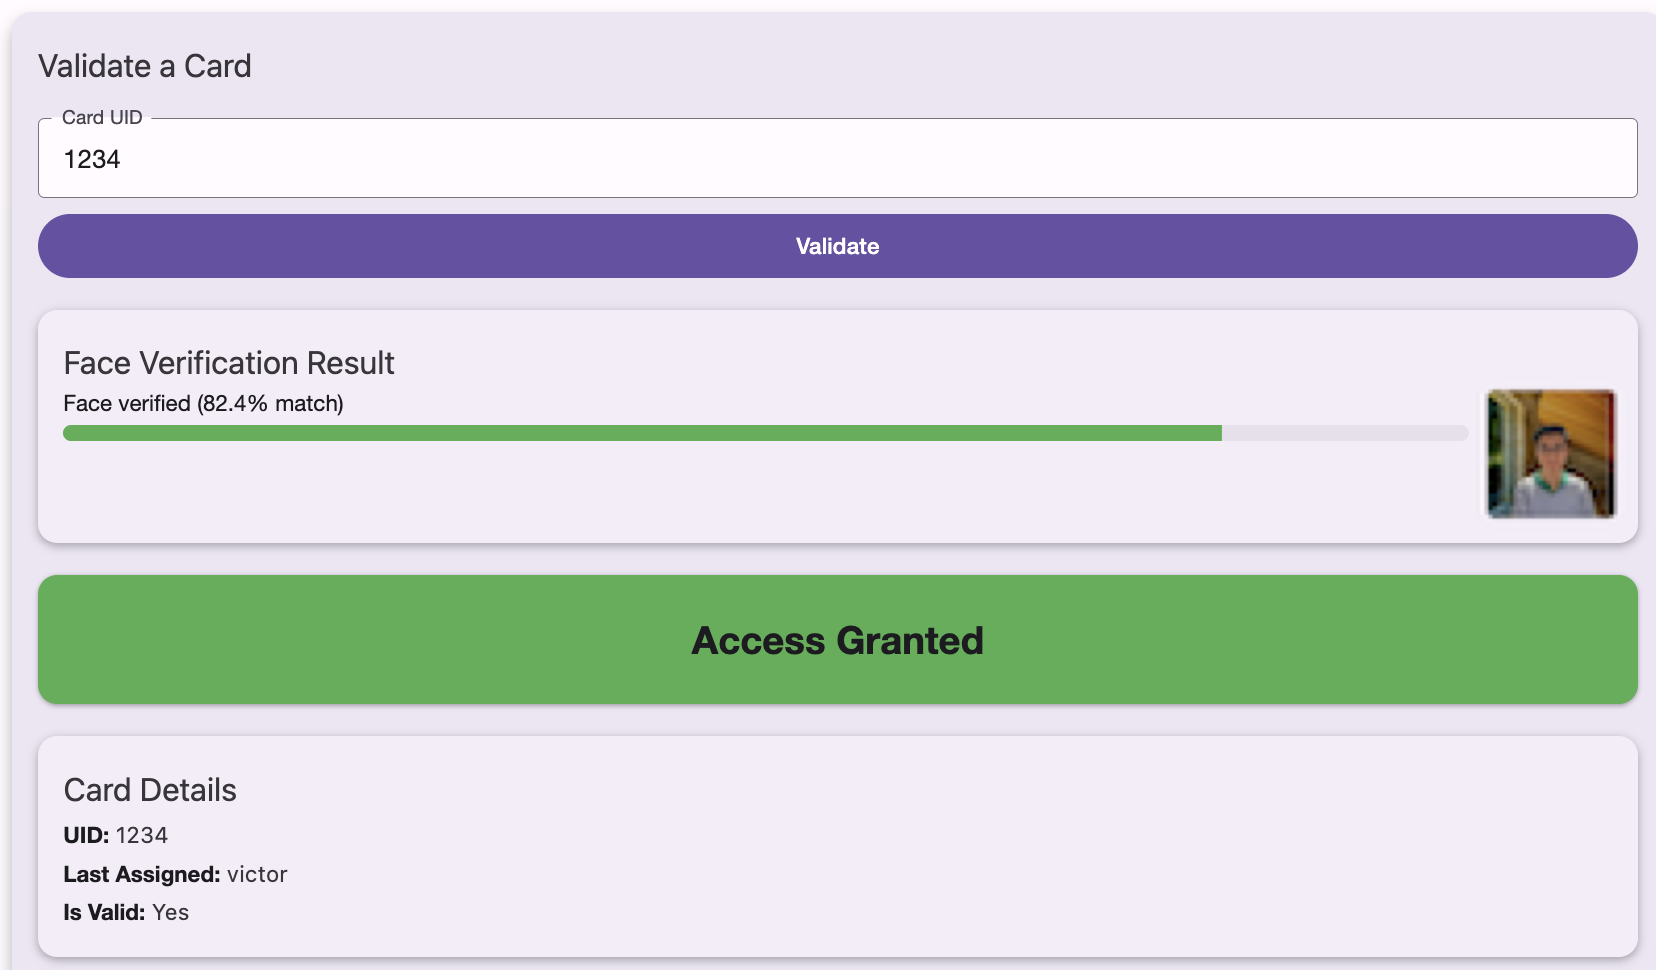
\includegraphics[width=0.8\textwidth,height=0.4\textheight,keepaspectratio]{figures/GuardAccessGranted.png}
  \caption{Benutzeroberfläche der Guard-App bei erfolgreicher Validierung}
  \label{fig:screenshot_guard}
\end{figure}

\subsection{Technische Artefakte}
Hier werden zentrale Code-Ausschnitte dokumentiert, die die technische Logik des Systems repräsentieren.

\subsubsection{Distanzberechnung (Euklidische Distanz)}
Die Entscheidung über eine Gesichtsübereinstimmung basiert auf der euklidischen Distanz der Face-Descriptoren.
\begin{lstlisting}
const distance = faceapi.euclideanDistance(
  snapshotDetection.descriptor,
  referenceDetection.descriptor
);
const threshold = 0.6;
const match = distance < threshold;
\end{lstlisting}

\subsubsection{HEIC-Konvertierungspipeline}
Die Normalisierung von iOS-Fotos erfolgt serverseitig durch eine Pipeline aus \texttt{heic-convert} und \texttt{sharp}.
\begin{lstlisting}
if (isHeicFormat || isHeifFormat) {
  heicBuffer = await heicConvert({
    buffer: imageBuffer,
    format: 'PNG',
    quality: 1
  });
  processedImageBuffer = Buffer.from(heicBuffer);
}
// Resize mit sharp auf Standardmass
const sharpOutput = await sharp(processedImageBuffer)
  .resize(1024, 1024, { fit: 'cover' })
  .png()
  .toBuffer();
\end{lstlisting}

\subsubsection{JWT-Authentifizierungs-Middleware}
Die Absicherung der Endpunkte erfolgt rollenbasiert mittels JSON Web Tokens.
\begin{lstlisting}
const checkAuth = (db, requiredPermissions = []) => {
  return (req, res, next) => {
    const token = req.headers.authorization.split(' ')[1];
    try {
      const decoded = jwt.verify(token, process.env.JWT_SECRET);
      req.user = decoded;
      if (requiredPermissions.length > 0) {
        const userPermissions = req.user.permissions || [];
        const hasPermission = requiredPermissions.every(p => userPermissions.includes(p));
        if (!hasPermission) return res.status(403).json({ error: 'Forbidden' });
      }
      next();
    } catch (err) {
      return res.status(401).json({ error: 'Unauthorized' });
    }
  };
};
\end{lstlisting}

\section{Anhang B: Reproduzierbarkeit und Projektlogik}

\subsection{Projektstruktur}
Das Projekt ist in zwei Hauptkomponenten unterteilt: das Node.js-Backend und das React-Native-Frontend. Die folgende Struktur zeigt die wesentlichen Verzeichnisse.
\begin{lstlisting}[language=bash]
.
|-- Backend/school-access-control-backend/
|   |-- middleware/ (Authentifizierung & Sicherheit)
|   |-- routes/ (API-Endpunkte)
|   |-- utils/ (Bildverarbeitung & KI-Logik)
|   |-- weights/ (TensorFlow.js Modellgewichte)
|   `-- server.js (Haupteinstiegspunkt)
|-- Frontend/SchoolAccessControl/ (Mobile App)
|-- BLL-LaTeX/ (Dokumentation)
`-- database.db (SQLite-Datenbank)
\end{lstlisting}

\subsection{Reproduktionsanleitung}
Um das System in einer Testumgebung zu reproduzieren, sind die folgenden Schritte notwendig.

\subsubsection{Hardware-Voraussetzungen}
\begin{itemize}
  \item Raspberry Pi 4 (mind. 4GB RAM empfohlen für KI-Inferenz)
  \item USB-RFID-Lesegerät (125\,kHz, EM4100-kompatibel)
  \item Kamera-Modul oder USB-Webcam zur Gesichtserfassung
\end{itemize}

\subsubsection{Software-Voraussetzungen und Installation}
\begin{enumerate}
  \item Installation von Node.js 22.x und npm.
  \item Repository klonen: \texttt{git clone <repository-url>}.
  \item Backend-Abhängigkeiten installieren:
    \begin{lstlisting}[language=bash]
    cd Backend/school-access-control-backend
    npm install
    npm rebuild @tensorflow/tfjs-node --build-from-source
    \end{lstlisting}
  \item Umgebungsvariablen konfigurieren: Datei \texttt{.env} mit \texttt{JWT\_SECRET} und \texttt{PORT=3000} anlegen.
  \item Server starten: \texttt{node server.js}.
\end{enumerate}

\subsubsection{Durchführung von Benchmarks}
Die im \autoref{sec:ergebnisse} (\nameref{sec:ergebnisse}) genannten Latenzwerte können durch die bereitgestellten Benchmark-Skripte verifiziert werden.
\begin{lstlisting}[language=bash]
cd Backend/school-access-control-backend/benchmarks
node benchmark_face.js
\end{lstlisting}
Das Skript gibt die Inferenzzeit für 20 Testbilder aus und speichert die Ergebnisse in \texttt{results/rpi\_face.csv}.

\subsection{Fehlerbehandlung und Plausibilitätschecks}
\begin{itemize}
  \item \textbf{Modell-Ladefehler:} Falls die Gewichte in \texttt{/weights} fehlen, startet der Gesichtserkennungs-Service nicht. Prüfen Sie das \texttt{server.log} auf entsprechende Fehlermeldungen.
  \item \textbf{Speichermangel:} Bei der Verarbeitung vieler HEIC-Bilder auf einem Raspberry Pi kann es zu \enquote{Out of Memory} Fehlern kommen. Das System ist so konfiguriert, dass es nach jeder Bildkonvertierung \texttt{global.gc()} aufruft (erfordert Start mit \texttt{--expose-gc}).
  \item \textbf{Erwartete Ausgabe:} Ein erfolgreicher RFID-Scan liefert ein JSON-Objekt mit \texttt{"valid": true} und der \texttt{photoUrl} des Schülers zurück.
\end{itemize}


\end{document}
